\documentclass[16pt, A4Paper]{article}
\usepackage{blindtext}
\parindent=0pt
\usepackage[utf8]{inputenc}
\usepackage{graphicx}
\usepackage{caption}
\usepackage{geometry}
\usepackage{amsmath}
\usepackage[none]{hyphenat}

\title{CSE317 Assignment:1}
\author{Name: Iftekhar E Mahbub Zeeon \hspace{5 cm} ID: 1805038 }
\begin{document}
\maketitle

\noindent\makebox[\linewidth]{\rule{\paperwidth}{0.4pt}}

\section*{Bayesian Network}
\paragraph{A Bayesian network is a data structure that represents the dependencies among random variables. Bayesian networks have the following properties:}

\begin{itemize}
  \item These are directed graphs.
  \item Each node on the graph represents a random variable.
  \item An arrow from \textit{X} to \textit{Y} represents that \textit{X} is a parent of \textit{Y}. That is, the probability distribution of \textit{Y} depends on the value of \textit{X}.
  \item Each node \textit{X} has conditional probability distribution \textit{P(X $|$ Parents(X))}.
\end{itemize}

\section*{Example of a Bayesian Network}
\paragraph{Let’s consider an example of a Bayesian network that involves variables that affect whether we get to our appointment on time.}

\begin{figure}[htpb]
\centering
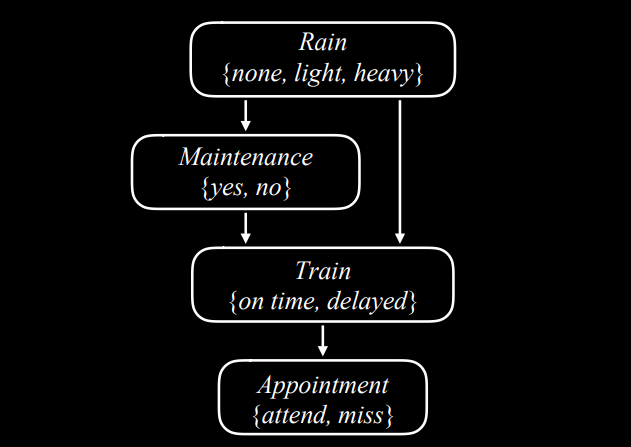
\includegraphics[width=300pt]{bayesian_network.png}
\caption{Bayesian Network}
\end{figure}

\subsection*{Probability Distribution of Rain}
\begin{center}
\begin{tabular}{ |c|c|c| } 
\hline
none & light & heavy \\
\hline
0.7 & 0.2 & 0.1 \\
\hline
\end{tabular}
\end{center}

\subsection*{Probability Distribution of Maintenance}
\begin{center}
\begin{tabular}{ |c|c|c| } 
\hline
R & yes & no \\
\hline
none & 0.4 & 0.6 \\
\hline
light & 0.2 & 0.8 \\
\hline
heavy & 0.1 & 0.9 \\
\hline
\end{tabular}
\end{center}

\subsection*{Probability Distribution of Train}
\begin{center}
\begin{tabular}{ |c|c|c|c| } 
\hline
R & M & on time & delayed \\ \hline
none & yes & 0.8 & 0.2 \\ \hline
none & no & 0.9 & 0.1 \\ \hline
light & yes & 0.6 & 0.4 \\ \hline
light & no & 0.7 & 0.3 \\ \hline
heavy & yes & 0.4 & 0.6 \\ \hline
heavy & no & 0.5 & 0.5 \\ \hline
\end{tabular}
\end{center}

\subsection*{Probability Distribution of Appointment}
\begin{center}
\begin{tabular}{ |c|c|c| } 
\hline
T & attend & miss \\ \hline
on time & 0.9 & 0.1 \\ \hline
delayed & 0.6 & 0.4 \\ \hline
\end{tabular}
\end{center}

\subsection*{Calculate prediction of maintenance based on the evidence that the train was delayed}
\begin{multline*}
P(maintenance | train=delayed) = \alpha [ P(delayed , maintenance , rain = none )+ \\
P(delayed , maintenance , rain = light)+ \\
P(delayed , maintenance , rain = heavy) ] \\
\end{multline*}
\begin{multline*}
= \alpha \langle \{ P (none) P(yes | none) P(delayed | yes , none) +\\ P(light) P(yes | light) P(delayed | yes , light) +\\
P(heavy) P(yes | heavy) P(delayed | yes , heavy) \} ,\\ \{ P(none) P(no | none) P(delayed | no , none) +\\
P(light) P(no | light) P(delayed | no , light) + \\ P(heavy) P(no | heavy) P(delayed | no , heavy) \}  \rangle \\
\end{multline*}
\begin{multline*}
= \alpha \langle  (0.7 * 0.4 * 0.2 + 0.2 * 0.2 * 0.4 + 0.1 * 0.1 * 0.6) , ( 0.7 * 0.6 * 0.1 + 0.2 * 0.8 * 0.3 + 0.1 * 0.9 * 0.5  )  \rangle
\end{multline*}
\begin{multline*}
= \alpha \langle  0.078 , 0.135  \rangle \\
\end{multline*}
\begin{multline*}
= \alpha \langle  0.3661 , 0.6338  \rangle \\
\end{multline*}
\begin{multline*}
  Where \alpha = 0.213 \\
 \textbf{ maintenance : }\\
  yes = 0.3661 \\
  no = 0.6338 \\
\end{multline*}

\subsection*{Calculate prediction of rain based on the evidence that the train was delayed}
\begin{multline*}
P(rain | train=delayed) = \alpha [ P(delayed , rain , maintenance = yes ) +\\ P(delayed , rain , maintenance = no ) ] \\
\end{multline*}
\begin{multline*}
 = \alpha \langle \{ P (none) P(yes | none) P(delayed | yes , none) +\\ P(none) P(no | none) P(delayed | no , none) \},\\ \{ P(light) P(yes | light) P(delayed | yes , light) +\\ P(light) P(no | light) P(delayed | no , light) \} ,\\ \{ P(heavy) P(yes | heavy) P(delayed | yes , heavy) +\\ P(heavy) P(no | heavy) P(delayed | no , heavy) \}  \rangle \\
 \end{multline*}
\begin{multline*}
 = \alpha \langle  (0.7 * 0.4 * 0.2 + 0.7 * 0.6 * 0.1) , ( 0.2 * 0.2 * 0.4 + 0.2 * 0.8 * 0.3 ) , ( 0.1 * 0.1 * 0.6 + 0.1 * 0.9 * 0.5 )  \rangle \\
 \end{multline*}
\begin{multline*}
  = \alpha \langle  0.098 , 0.064 , 0.051  \rangle \\
  \end{multline*}
\begin{multline*}
  = \alpha \langle  0.46 , 0.3 , 0.24  \rangle \\
  \end{multline*}
\begin{multline*}
  Where \alpha = 0.213 \\
  \textbf{ rain : }\\
  none = 0.46 \\
  light = 0.3 \\
  heavy = 0.24 \\
\end{multline*}

\section*{Result after running inference.py}
\begin{figure}[htpb]
\centering
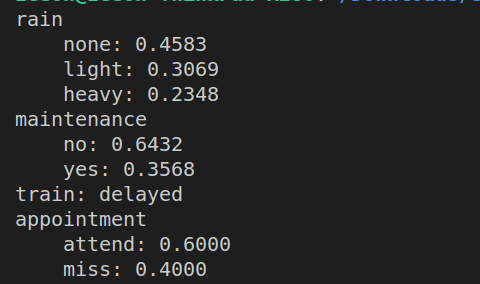
\includegraphics[width=200pt]{image.png}
\end{figure}
\end{document}
